\documentclass[a4paper,10pt]{article}
\usepackage[margin=0.5in]{geometry}
\usepackage[utf8]{inputenc}
\usepackage{amsmath}    % need for subequations
\usepackage{graphicx}   % need for figures
\usepackage{verbatim}   % useful for program listings
\usepackage{color}      % use if color is used in text

  % use for side-by-side figures
%\usepackage{hyperref}  
%opening
\title{Knowledge and Women}
\author{Shri Sruthi and Bama Srinivasan \\  Department of Computer Science and Engineering \\  Department of Information Science and Technology \\ CEG Campus \\Anna University Chennai}
\date{}

\begin{document}

\maketitle

\begin{abstract}
Since ancient times, women have been held at an esteemed position in terms of knowledge. This paper tries to address the role of women who have raised the scientific levels to great heights both from the Indian and Western Perspective. From the Indian perspective, Indians have regarded Goddess Saraswat\={i} as the mother of knowledge and wisdom. The intellectual calibre of Indian women has been explicitly stated in the epics and pur\={a}nas. From the western viewpoint,  there has been evidences of Greeks and Romans worshipping Goddess Athena and Minerva, respectively. These characters, albeit mythological portray the essence of the limitless capabilities of women. Starting from the historic times, India have seen remarkable individuals with scientific aptitude. A few of them are Gargi, Avvaiy\={a}r and L\={i}l\={a}vati. In the modern times, a few women excelled in the field of mathematics, physics, chemistry and medicine. Similarly, Egyptians, Greeks and Romans have had women professionals in the past. In 
the recent times, Ada Lovelace and Gracehopper have made breakthroughs in technology. This paper attempts to give a brief outlook of some of these individuals in the field of language, mathematics and science with a focus on knowledge. 
\end{abstract}
\section{Introduction}
From time immemorial, one of the traits that help to gauge a person is knowledge. The more knowledge a person has, the more respect she gets from the society. This knowledge can be straight away related to expertise in the varied fields, which encompass areas such as language, poetry, mathematics, science, technology, etc., 

Of late Science, Technology, Engineering and Mathematics (STEM) has shaped the world in a dramatic manner. A plethora of experts have worked endlessly and have made a breakthrough in the respective field. Among these experts, there are notable women who have broken the shackles of myth of gender suppression and proved their capabilities. This aspect can be seen worldwide, be it in India, Greece, USA, France or Italy. 

This paper lists a few remarkable women who made their way into their respective field of study. First, women in Historical period is described in Section \ref{sec:History}. This section includes Indian and western personalities. Section \ref{sec:modern} lists a few individuals in the area of STEM, both from India and abroad. Section \ref{sec:analysis} gives an overview of the different individuals and the respective field of study and Section \ref{sec:conclusion} concludes the paper. 

\section{Historical Period}
\label{sec:History}
In the past, the world has regarded the knowledge as the highest trait and the provider of knowledge is invariably Goddess Saraswat\={i} in India. Similarly other regions also have their Goddesses dedicated to knowledge and wisdom. The mythology also has a number of female personalities personifying the characteristics of knowledge. This section gives a brief account of a few such personalities who excelled in the past. First, Indians are specified, followed by the western individuals. 

\subsection{Indian Personalities}
In Vedic period, three Goddesses namely, \textbf{Illa, Saraswat\={i} and Mahi} have been quoted for the purpose of acquiring knowledge as \cite{saras}: \\
“May Bharati (Mahi) come speeding to our sacrifice and Ila hither awakening our consciousness in human wise, and Saraswat\={i}, — three goddesses sit on this blissful seat, doing well the Work.” \\

The image of the \textbf{Goddess Saraswat\={i}} (Figure 1) portrays a musical instrument called Veena holding in  two hands, a book in one hand and a tiny garland in another hand. These represent music, knowledge and inner bliss, respectively. 
\begin{center}
\begin{figure}[h]
\centering
 \includegraphics[scale=0.7]{saraswati.png}
 \caption{Goddess Sarawati}
\end{figure}
\end{center}

The Vedic period has seen intellectuals like \textbf{Gargi and Maitreyi}. Gargi Vachnaknavi, who lived during 700 BC was honored as a great philosopher \cite{Gargi}. The debate between Gargi and Yajnavalkya has been specified in Brihadaranyaka Upanishad, in which Gargi puts forth a series of thought provoking questions to Yajnavalkya. A few such questions from this debate are given below. \\

\textit{Yajnavalkya ,`` said she, ``if all this is pervaded by water, by  what, pray, is water pervaded?''} \\
\textit{``By air, O Gargi.", replied Yajnavalkya.} \\
\textit{``By what, pray, is air pervaded?" }\\
\textit{``By the sky, O Gargi."} \\
\textit{``By what is the sky pervaded?"}  \\

These questions clearly indicate depth of thought that Women possess. On a similar front, in the Indian Epic Mahabharatha, there are instances of women empowerment. \textbf{Draupadi} is known to have managed the people and wealth in the palace \cite{mahabharatha}. 

In South India, around First or Second Century A.D. there was a Tamil Poet called \textbf{Avvaiy\={a}r}. In one of her poems, she specifies about the information of energy of an atom as \\
\begin{center}
``aNuvaith thuLaiththu Ez kadalai puguththi'' \\
\textit{Energy of seven seas within a pierced atom}\\
\end{center}
This line indicates the level of scientific thought process in those days. 

\textbf{L\={i}l\={a}vati} was the daughter of Bhaskara (during 1150 A.D), who was one of the pioneers in Indian mathematics. The tale goes like this: L\={i}l\={a}vati was an intelligent and inquisitive child and Bhaskara had always kept an eye on this nature of hers. However, when Bhaskara analysed her horroscope, he was shocked to see that her marriage will be short-lived. To circumvent this issue, Bhaskara prepared a perfect device that could calculate the auspicious time for her marriage. L\={i}l\={a}vati's curiousness drew her close to the device (when her father was not near) and while examining, the pearl that she was wearing fell into the device. The calculations went awry and the auspicious time was missed. Eventually, L\={i}l\={a}vati got married, but as feared it was short-lived. Soon after this incidence, L\={i}l\={a}vati was extremely upset and was not able to lead her regular normal activities. In order to overcome her worries, Bhaskara posed a lot of arithmeic puzzles which made her busy. These 
questions later on helped her to be the 
greatest mathematicians of all times \cite{lilavati}. 

\subsection{Western Personalities}
\newblock
According to the Greek Mythology, \textbf{Athena} is the embodiment of wisdom and power.\\
Various poems written for her by Odysseus G. Osborne spot light the depth of powers that the Goddess has.\\
\begin{center}
\begin{figure}[h]
\centering
 \includegraphics[scale=0.7]{athena_7.jpg}
 \caption{Goddess Athena}
\end{figure}
\end{center}

One of the many poems written on Athena in relation to Wisdom as \cite{athena}:\\
\begin{center}
\textit{Marshal of Wisdom}\\
\textit{give the gift as you resolve,}\\
\textit{As a Lance of Glory,}\\
\textit{Heralding your puissant strike!}\\
\textit{Or like a silent owl}\\
\textit{A glide on the Nights wind}\\
\textit{With talons wide!}\\
\textit{Mighty Athena! Let me be re-born of your thunderbolt!}\\
\end{center}

\newblock
\textbf{Minerva} was the Roman Goddess of Wisdom and war. She is believed to be the inventor of numbers and musical instruments. She was later equated with the Greek Goddess of Wisdom, Athena. She was called as the “goddess of thousand works” by Ovid, a Roman poet. She was being worshipped on the Capitoline Hill along with Jupiter and Juno as the Powerful triad of Gods.

\newblock
Mythologically According to Homer, \textbf{Agamede} was a Greek physician acquainted with the healing powers of all the plants that grow upon the earth.\\

\newblock
\textbf{Merit-Ptah} is believed by Egytologists to be the first-ever named Physician. She is most notable for being the first woman known by name in the history of the field of medicine, and also the first named woman in all of science as well.\\

She practiced medicine nearly 5,000 years ago, and was immortalized by her son on her tomb as “the chief physician”\cite{merit}.
\begin{center}
\begin{figure}[h]
\centering
 \includegraphics[scale=0.7]{meritptah.jpg}
 \caption{Merit Ptah}
\end{figure}
\end{center}

\newblock
\textbf{Agnodike} was the first female Athenian physician, midwife, gynaecologist. She studied in Alexandria under the great Herophilos, the first anotomist.

\begin{center}
\begin{figure}[h]
\centering
 \includegraphics[scale=0.7]{agnodice.jpg}
 \caption{Agnodike}
\end{figure}
\end{center}

\newblock
\textbf{Maria the Jewess} are the first female alchemist and is credited with the invention of several chemaical apparatus.

\newblock
\textbf{Hypatia} was a Greek mathematician, astronomer and philosopher in Egypt. She was the head of Neoplatonic school of Alexandria. Her contributions are considered as invention of the hydrometer used to determine the relative density (or specific gravity) of liquids. She worked collaboratively with her father on many works.\\

\section{Modern Period}
\label{sec:modern}
Notable women have shown the expertise in medicine, physics, botany, chemistry, mathematics and technology. This section provides a description of such women who excelled in the fields of STEM from India and abroad. 
\subsection{Scientific women personalities from India}
\newblock
\textbf{Janaki Ammal Edavaleth Kakkat} (4 November 1897 – 7 February 1984) was the botanist whose works are considered to be one of the most important breakthroughs in the research of sugarcane and eggplant. Having born and brought up in Kerala, she pursued school and college education in her home town and Chennai, respectively. She then went to USA to receive the doctorate during 1931. She is considered to be the first woman to obtain a Ph.D in botany from USA. A flower has also been named after her as 'Magnolia Kobus Janaki Ammal' \cite{janaki}.

\newblock
\textbf{Aseema Chatterjee (1917 - 2006)} was a notable Indian chemist in the area of organic chemistry and phytomedicine. She received M.Sc in the field of Organic Chemistry in 1938 and D.Sc. from the same university in 1944. ``She made significant contributions in the field of medicinal chemistry with special reference to alkaloids, coumarins and terpenoids, analytical chemistry, and mechanistic organic chemistry''.  \cite{chaterjee}


\newblock
\textbf{Dr. Anandi Gopal Joshi (1865 - 1887)} was the first female to obtain the medicine degree from USA. It was during the time of when Britain ruled India and hence Indians had an awareness of science from the west. As a regular practice those days, children were married at an early age and Anandi was not an exception. Her Husband Gopal Joshi encouraged Anandi to pursue education. She gave birth to a boy while she was fourteen years. But due to the non-availability of medical facilities, the baby could not survive beyond 10 days. This prompted her to pursue medicine and her husband helped her to send to USA for a medical profession. Despite her challenges of poor health, she successfully completed MD in 1886. She returned back to India on 1887 and wanted to open a medical college for women in India. But her health declined and died in 1887  \cite{joshi}.

\newblock
\textbf{Shakuntala Devi (1929 - 2013)} was the arithmetic prodigy of the century. She is known as the ``human computer'', since she could calculate even a 13X13 digit multiplication in 28 seconds. Her father was a working in a circus and had taught her card tricks, which enabled him to discovered the mathematical trait in her. She did not have a formal school education because of financial constraints. However, it does not deter the spirit of Shakuntala Devi to pursue the love for numbers. She travelled across widely to Europe and USA and exhibited her talent. Her calculation approach was appreciated by the scholars worldwide and her multiplication of 13X13 number was recorded in Guiness Book of Records \cite{shakuntala}. 

\newblock
\textbf{Anna Mani (1918 - 2001)} was a physicist and a meterologist, who made important contributions in meterological instrumentation. She was influenced in her younger days by Gandhian movement and vowed to wear kh\={a}di, a typical variety of cloth made by Indians. She initially wanted to pursue medicine, but shifted her career to physics since it appealed her more. She pursued her degree from Presidency college and did research under Sir.C.V. Raman. Since she did not have masters degree, she could not get Ph.D at that time. She then proceeded to Imperial college, London for a degree in meterological studies and then returned back to India. She was the deputy director of Indian Meterological department and authored a number of papers in the area of meterological instrumentation. \cite{anna}

\textbf{Dr. Muthulakshmi Reddy (July 1886 – 22 July 1968)} was one of the pioneers in India to be the first in many sectors: ``first female student to be admitted into a men's college, the first woman House Surgeon in the Government Maternity and Ophthalmic Hospital, the first woman legislator in British India, the first Chairperson of the State Social Welfare Advisory Board, the first woman Deputy President of the Legislative Council, and the first Alderwoman of the Madras Corporation Avvai Home'' \cite{reddy}. Despite the pressure of stopping the education citing gender as a reason, Dr. Muthulakshmi stood against odds and completed the degree of medicine from Madras Medical College. She did not stop there, but entered into political career and also was a social reformer. Her proof of success stands today as Adayar Cancer Institute, which she initiated for the benefit of masses. This reform is presently headed out by another female physician namely, Dr.Shantha \cite{shantha}. 


\subsection{Scientific women personalities from the western world}
\newblock
Christine de Pizan is a fifteenth-century writer in France. She is the author of the Book of the City of the Ladies. She was an early feminist who challenged her culture's stereotypes of women.She wrote love ballads, books supporting and extolling the powers and virtues of women (including a response to Jean de Meun's Roman de la rose), and a work about Joan of Arc.\cite{christine}\\

\begin{center}
\begin{figure}[h]
\centering
 \includegraphics[scale=0.2]{christine.jpg}
 \caption{Christine de Pizan}
\end{figure}
\end{center}

\newblock
\\
Maria Sibylla Merian was a Naturalist, an Entymologist and a Botanical Illustrator. She published collections of engravings of plants in 1675, 1677, and 1680. She collected and observed live insects and created detailed drawings to illustrate insect metamorphosis.\cite{merian}


\begin{center}
\begin{figure}[h]
\centering
 \includegraphics[scale=0.4]{maria.jpg}
 \caption{Maria Sibylla Merian}
\end{figure}
\end{center}


\newblock
Maria Gaetana Agnes was the first woman to write a mathematics handbook and the first woman appointed as a Mathematics Professor at a university.She is credited with writing the first book discussing both differential and integral calculus and was a member of the faculty at the University of Bologna\cite{agnesi}.

\begin{center}
\begin{figure}[h]
\centering
 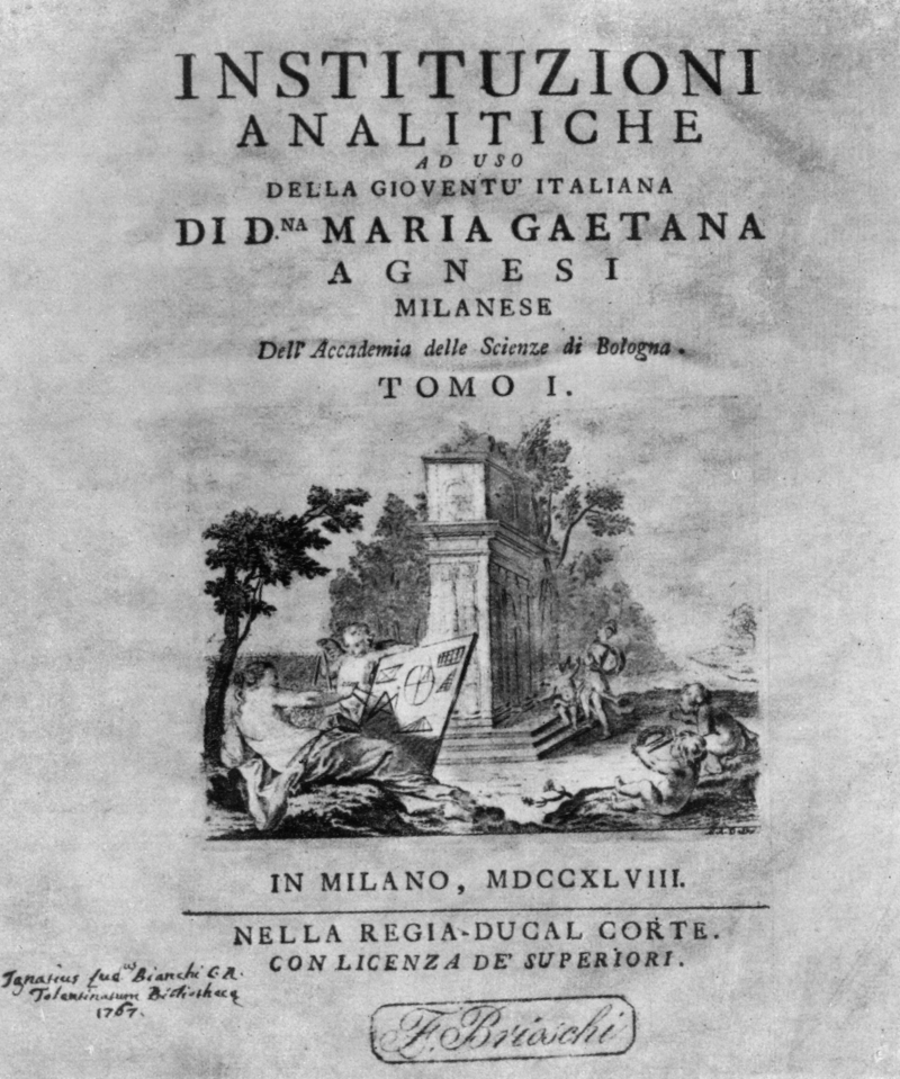
\includegraphics[scale=0.9]{agnesi.png}
 \caption{First Page of the Book Agnesi wrote}
\end{figure}
\end{center}

\newblock
Laura Bassi was an Italian scientist and the first woman professor to be appointed at a European university\cite{laura}.

\begin{center}
\begin{figure}[h]
\centering
 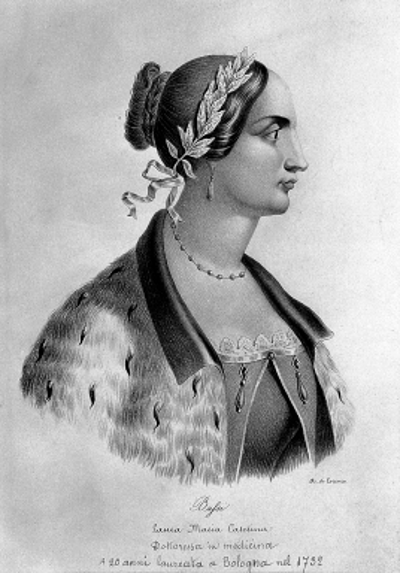
\includegraphics[scale=0.9]{laura.png}
 \caption{Laura Bassi}
\end{figure}
\end{center}

\newblock
Charlotta Frolich became the first of her gender to be published by the Royal Swedish Academy of Sciences with three books in agricultural science depicting her own experiences and suggesting various inventions in agriculture. The only other female to be published by the Academy of Sciences during the age of liberty was Eva Ekeblad\cite{frolich}.

\begin{center}
\begin{figure}[h]
\centering
 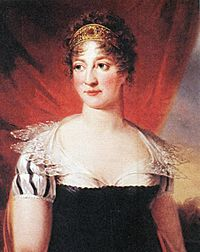
\includegraphics[scale=0.7]{charlotta.jpg}
 \caption{Charlotta Frolich}
\end{figure}
\end{center}

Marie Curie

Ada Lovelace

Grace Hopper

\section{Analysis}
\label{sec:analysis}
The biographies of each of the aforementioned individuals provide the proof of the accompolishment in varied fields. An analysis in terms of the field and the challenges that they faced are provided in Table \ref{tab:analysis}.
\begin{table}
\label{tab:analysis}
\caption{Analysis of a few female personalities}
\centering
 \begin{tabular}{|l|l|l|l|l|}
  \hline
  S.No & Name & Period & Area of Excellence & Challenges Faced \\
  \hline
 
 \end{tabular}

\end{table}


\newblock
Name : \\
Period : \\
Area of Excellence : \\
Challenges faced : \\

\newblock
Name : \\
Period : \\
Area of Excellence : \\
Challenges faced : \\

\newblock
Name : \\
Period : \\
Area of Excellence : \\
Challenges faced : \\

\newblock
Name : \\
Period : \\
Area of Excellence : \\
Challenges faced : \\

\newblock
Name : \\
Period : \\
Area of Excellence : \\
Challenges faced : \\

\newblock
Name : \\
Period : \\
Area of Excellence : \\
Challenges faced : \\

\newblock
Name : \\
Period : \\
Area of Excellence : \\
Challenges faced : \\

\newblock
Name : \\
Period : \\
Area of Excellence : \\
Challenges faced : \\

\newblock
Name : \\
Period : \\
Area of Excellence : \\
Challenges faced : \\

\newblock
Name : \\
Period : \\
Area of Excellence : \\
Challenges faced : \\

\newblock
Name : \\
Period : \\
Area of Excellence : \\
Challenges faced : \\

\newblock
Name : \\
Period : \\
Area of Excellence : \\
Challenges faced : \\

\newblock
Name : \\
Period : \\
Area of Excellence : \\
Challenges faced : \\

\newblock
Name : \\
Period : \\
Area of Excellence : \\
Challenges faced : \\

\section{Conclusion}
\label{sec:conclusion}
This paper has provided a list of few intellectual women who were successful in their field of study. The enormous struggles and hardship that these women have faced cannot be accounted in a single article. With limited resources and support, the women went on to become pioneers in their respective field. For example, Dr. Anandi had faced difficulties in multiple dimensions - in terms of gender, money, health and religion. But these factors does not deter her towards her goal. Same is the case with other women personalities. In the present scenario, given the choices of facilities and technology, there is no limit to reach great heights in STEM. With this little background, we hope that this paper will act as an inspiration to the present generation female individuals.
\begin{thebibliography}{9}

\bibitem{saras}
http://www.universityofhumanunity.org/biblios/Sarasvati%20in%20the%20Veda%20-%20Part%201.pdf

\bibitem{Gargi}
Ahuja, M.L. 
\newblock {2011.}
\newblock { Women in Indian Mythology}
\newblock {Rupa Publications}

\bibitem{mahabharatha}
 Kisari Mohan Ganguli
\newblock{The Mahabharata of Krishna-Dwaipayana Vyasa}
\newblock{Translation from original Sanskrit Text}
\newblock{http://sacred-texts.com/hin/maha/index.htm}

\bibitem{athena}
https://sites.google.com/site/shrineathenapromachos/prayers-poems

\bibitem{merit}
http://www.ancient.eu/article/49/

\bibitem{christine}
http://historymedren.about.com/od/cwho/a/Christine-De-Pizan-Quotes.htm

\bibitem{merian}
https://en.wikipedia.org/wiki/Maria\_Sibylla\_Merian

\bibitem{agnesi}
https://en.wikipedia.org/wiki/Maria\_Gaetana\_Agnesi

\bibitem{laura}
http://www.sciencemuseum.org.uk/broughttolife/people/laurabassi

\bibitem{frolich}
https://alchetron.com/Charlotta-Frolich-1083211-W

\bibitem{lilavati}
\newblock{Retreived from http://4go10tales.blogspot.in/2012/06/lilavati.html}

\bibitem{janaki}
\newblock{Retreived from https://en.wikipedia.org/wiki/Janaki\_Ammal}

\bibitem{chaterjee}
by S C Pakrashi.
\newblock{Asima Chatterjee},
\newblock{Retreived from http://www.ias.ac.in/public/Resources/Initiatives/Women\_in\_Science/Contributors/Chatterjee.pdf}

\bibitem{joshi}
Dall, Caroline Wells Healey,
\newblock{The life of Dr. Anandabai Joshee: A kinswoman of the Pundita Ramabai}
\newblock{Roberts Brothers (Boston, Mass.), 1888}

\bibitem{shakuntala}
\newblock{Shakuntala Devi, ‘Human Computer’ Who Bested the Machines, Dies at 83, The NewYork Times', Retreived from http://www.nytimes.com/2013/04/24/world/asia/shakuntala-devi-human-computer-dies-in-india-at-83.html}

\bibitem{anna}
\newblock{Retreived from http://www.thebetterindia.com/83063/anna-mani-scientist-meteorology-ozone-wind-energy/}

\bibitem{reddy}
\newblock{Retreived from https://en.wikipedia.org/wiki/Muthulakshmi\_Reddi}

\bibitem{shantha}
\newblock{Retreived from http://health.economictimes.indiatimes.com/news/hospitals/interview-dr-v-shanta-chairperson-cancer-institute-wia-adyar-chennai/49182834}



\end{thebibliography}

\end{document}
